% !TeX root = ../main.tex

% \appendixtoc
% \appendix
% \ohead[]{\textsc{Appendix}}
\label{app:appendix}

% \renewcommand\thechapter{\roman{chapter}}
% \setcounter{chapter}{0}

% \pagebreak
% \includepdf[pages=-,scale=.9,pagecommand={}]{Aufgabenstellung.pdf} 
% PDF um 10% verkleinert einbinden --> Kopf- und Fußzeile  werden so korrekt dargestellt. Die Option `pages' ermöglicht es, eine bestimmte Sequenz von Seiten (z.B. 2-10 oder `-' für alle Seiten) auszuwählen.
% \pagebreak
%\includepdf[pages=-,scale=.8,pagecommand=\section*{A. eventGenerator.py}]{../appendix/eventGenerator.py.pdf}
%\includepdf[pages=-,scale=.8,pagecommand=\section*{B. sendEvents.py}]{../appendix/sendEvents.py.pdf}


% \RedeclareSectionCommand[beforeskip=\kapitelabstand         ]{chapter}


%%%%%%%%%%%%%%%%%%%%%%%%%%%%%%%%%%%%%%%%%%

%%%%%%%%%%%%%%%%%%%%%%%%%%%%%%%%%%%%%%%%%%
%%%%%%%%%%%%%%%%%%%%%%%%%%%%%%%%%%%%%%%%%%
\chapter{Fundamentals}

\section{Voltage Stability Basics: Definitions}
\label{app:voltage-stability-definitions}

All of the follwong definitions are direct citations, and therefore the same wording as in the paper of \textcite{shoup_2004}. 
The definitions are short, precise and summarized resp. sythesized from papers and report from \ac{CIGRE}\footnote{french for International Council on Large Electric Systems} and \ac{IEEE}.

\textbf{Voltage dip:}
\begin{quote}\itshape
    A temporary reduction of the voltage at a point in the electrical system below a threshold. 
    If during a voltage dip the voltage falls below an interruption threshold, the event is sometimes considered to be both a dip and an interruption.
\end{quote}

\textbf{Voltage sag:}
\begin{quote}\itshape
    An rms variation with a magnitude between 10 \% and 90 \% of nominal and a short duration between 0.5 cycles and one minute.
\end{quote}

\textbf{Power system stability:}
\begin{quote}\itshape
    Power system stability is the ability of an electric power system, for a given initial operating condition, to regain a state of operating equilibrium after being subjected to a physical disturbance, with most system variables bounded so that practically the entire system remains intact.
\end{quote}

\textbf{Voltage stability:}
\begin{quote}\itshape
    Voltage stability refers to the ability of a power system to maintain steady voltages at all buses in the system after being subjected to a disturbance from a given initial operating condition. 
    It depends on the ability to maintain/restore equilibrium between load demand and load supply from the power system. 
    Instability that may result occurs in the form of a progressive fall or rise of voltages of some buses. 
    A possible outcome of voltage instability is a loss of load in an area, or tripping of transmission lines and other elements by their protective systems leading to cascading outages. 
    Loss of synchronism of some generators may result from these outages or from operation under field current limit.
\end{quote}

\textbf{Short-term voltage stability:}
\begin{quote}\itshape
    Short-term voltage stability involves dynamics of fast acting load components such as induction motors, electronically controlled loads and HVDC converters. 
    The study period of interest is in the order of several seconds, and analysis requires solutions of appropriate system differential equations; that is similar to analysis of rotor angle stability. 
    Dynamic modeling of loads is often essential. 
    In contrast to angle stability, short-circuits near loads are important. 
    The term transient voltage stability is deprecated.
\end{quote}

\section{Comparison of Trigonometric Functions}
\label{app:trogonometric-func-comp}

\begin{figure}[H]
    \centering
    % \missingfigure{Comparison Tan, Cos, and Sin}
    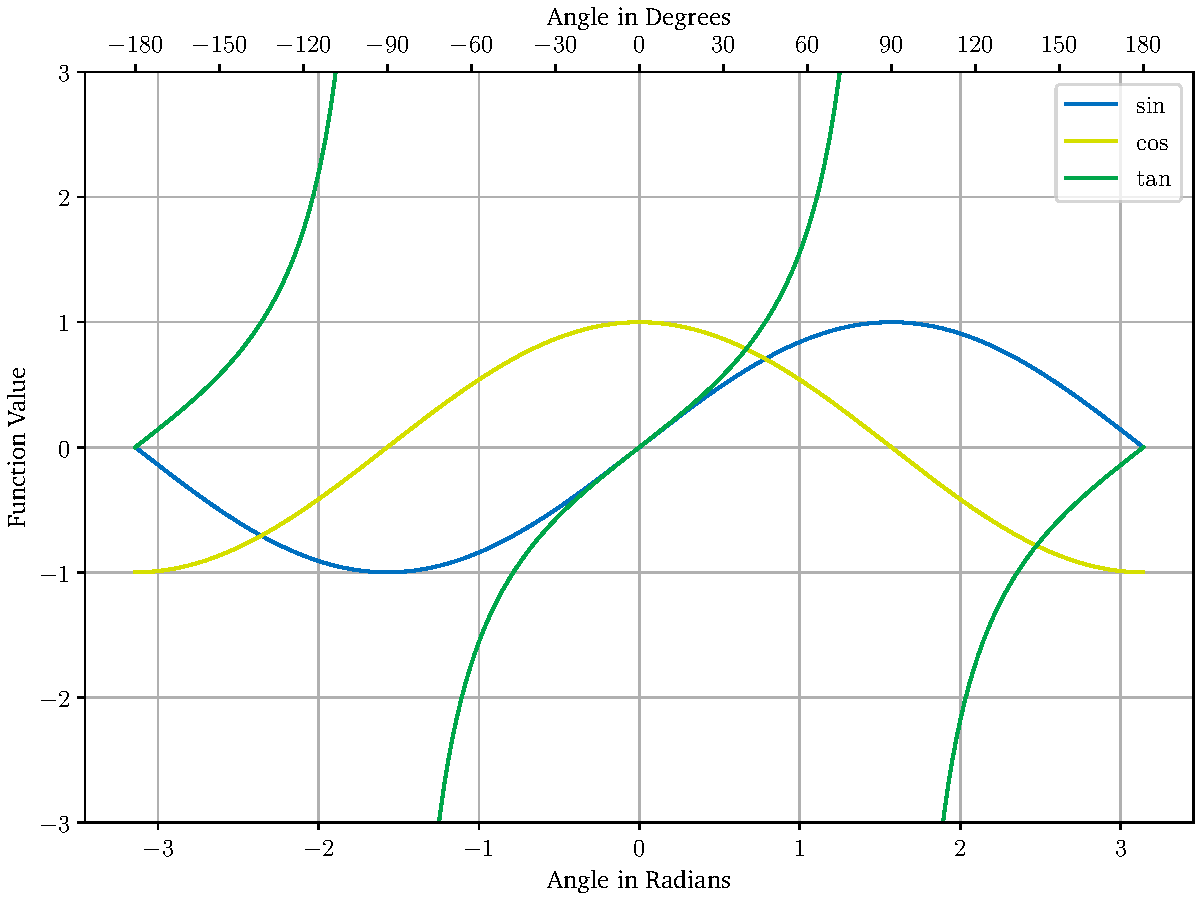
\includegraphics[width=\linewidth]{plots/trigonometric_functions.pdf}
    \caption[Plot comparison of trigonometric functions]{Plot comparison of trigonometric functions}
    \label{fig:trigonometric-func}
\end{figure}

Trigonometric functions are used as relation between apparent power $S$, active $P$ and reactive power $Q$.
While in discription of dynamics, the planning of networks or connection of machines, often the cosinodal function and therefore its value is present in the feeling of (engineering) people.
In stability analysis often the $\tan$ function is used, simply because its directly connecting onle active and reactive power, and because some athematic reformulations are possible with that. 
\autoref{fig:trigonometric-func} is illustrating relations of these functional values to the angle in rad and degree, while \autoref{tab:trigonometric-func} gives a numerical connection.
This shall increase the feeling and evaluation of this thesis readers.

\begin{table}[H]
    \centering
    \small
    \caption{Comparison of trigonometric functions dependent on the angle $\phi$ in degree or radians}
    \label{tab:trigonometric-func}
    \vspace*{12pt}
    \begin{tabularx}{\linewidth}{XXXXX}
        \textbf{Angle in $^\circ$} & \textbf{Angle in rad} & \textbf{$\sin$} & \textbf{$\cos$} & \textbf{$\tan$} \\ \toprule
        0   & 0         & 0         & 1         & 0 \\
        10  & 0.1745    & 0.1736    & 0.9848    & 0.1763 \\
        20  & 0.3490    & 0.3420    & 0.9397    & 0.3640 \\
        30  & 0.5236    & 0.5       & 0.8660    & 0.5774 \\
        40  & 0.6981    & 0.6428    & 0.7660    & 0.8391 \\
        50  & 0.8727    & 0.7660    & 0.6428    & 1.1918 \\ 
        60  & 1.0472    & 0.8660    & 0.5       & 1.7321 \\
        70  & 1.2217    & 0.9397    & 0.3420    & 2.7475 \\
        80  & 1.3962    & 0.9848    & 0.1736    & 5.6713 \\
        90  & 1.5708    & 1         & 0         & $\nexists$ \\
        120 & 2.0944    & 0.8660    & -0.5      & -1.7321 \\
        150 & 2.6180    & 0.5       & -0.8660   & -0.5774 \\
        180 & 3.1416    & 0         & -1        & 0 \\
        \bottomrule
    \end{tabularx}
\end{table}

\section{Description of the Power System Simulation process}
\label{app:power-system-modeling}

In this appendix section, the general process of power system simulation is described. As this thesis is aiming to understand voltage stability and processes in longer periods of time, these explanations apply to pointer-based simulations, called RMS simulations. Meaning that the considered effects are slower electromechanical nature instead of faster electromagnetic ones. The in this thesis used Python framework \glqq \textit{diffpssi}\grqq~is based on this type of simulation, and due to its open-source based nature traceable.

\begin{figure}[H]
    \centering
    % \includegraphics[width=\textwidth]{fundamentals/power-system-simulation-process.pdf}
    \missingfigure{Power system simulation process}
    \caption{Power system simulation process; own illustration}
    \label{fig:power-system-simulation-process}
\end{figure}

\commenting{
    Really basic: (?)
    \begin{itemize}
        \item RMS vs EMT simulation (-> meaning one cannot simulate other faults than 3ph w/o ground)
        \item Phasor description
        \item Basic formulation: Static (algebraic) and dynamic (differential) equations
        \item Using of solvers (Integrators) for time domain simulation
        \item Using of different optimizatinon algorithms for steady state (load flow) simulation -> initial values
    \end{itemize}
    Less basic and more advanced:
    \begin{itemize}
        \item rountines in the framework
        \item two types: Algebraic and Differential equations have to be solved at each time step -> What is which? Which operational equipment is typically described with which type of equation?
        \item per unit system applying for easier simulation (different voltage levels)
        \item ...
    \end{itemize}
}

%%%%%%%%%%%%%%%%%%%%%%%%%%%%%%%%%%%%%%%%%%
% \section{Jacobian based voltage stability criterions}
% \label{app:jacobian-voltage-indices}

% \textcite{danish_2015} is showing, describing, and referencing some voltage stability indices based on the Jacobian matrix. The following table is a collection of these indices.

% \begin{sidewaystable}[H]
%     \centering
%     \small
%     \caption{Jacobian based voltage stability criterions; after \textcite{danish_2015}}
%     \vspace*{12pt}
%     \renewcommand{\arraystretch}{2}
%     \begin{tabularx}{23cm}{llXXl}
%         % \toprule
%         \textbf{Index} & \textbf{Abbreviation} & \textbf{Calculation} & \textbf{Stability Threshold} & \textbf{Reference} \\
%         \toprule
%         Tangent Vector Index & \acs{TVI} & $\mathrm{TVI}_i=\left\lvert \frac{\dd{V_i}}{\dd{\lambda}}\right\rvert^{-1}$ & depending on load increase & \\ \midrule
%         Test Function & & $t_{cc}=\left\lvert e^T_c \cdot \mab{J} \times \mab{J}_{cc}^{-1} \cdot e_c\right\rvert$ & details are given in reference & \\ \midrule
%         Second Order Index & $i$ & $i=\frac{1}{i_0} \cdot \sigma_\mathrm{max} \cdot \big( \dv{\sigma_\mathrm{max}}{\lambda_\mathrm{total}} \big)^{-1}$ & $i > 0$ & \\ \midrule
%         Minimum Eigenvalue & & $\Delta V=\sum_{i} \frac{\xi_i\eta_i}{\lambda_i} \Delta Q$ & all eigenvalues should be positive & \\ \midrule
%         Minimum Singular Value & & $\begin{bmatrix} \Delta \vartheta \\ \Delta V \end{bmatrix}=\mab{V} \sum^-1 \mab{U}^T \begin{bmatrix} \Delta F \\ \Delta G \end{bmatrix}$ & details are given in reference & \\ \midrule
%         Predicting Voltage Collapse & & $\frac{V}{V_0}$ & the smallest index value & \\ \midrule
%         Impedance Ratio & & $\frac{Z_ii}{Z_i}$ & $\frac{Z_ii}{Z_i} \leq 1$ & \\
%         \bottomrule
%     \end{tabularx}
% \end{sidewaystable}



% %%%%%%%%%%%%%%%%%%%%%%%%%%%%%%%%%%%%%%%%%%
% \section{Comparison of System based and Jacobian based indices}
% \label{app:jacobian-vs-system-indices}

% %%%%%%%%%%%%%%%%%%%%%%%%%%%%%%%%%%%%%%%%%%
% %%%%%%%%%%%%%%%%%%%%%%%%%%%%%%%%%%%%%%%%%%
\chapter{Modeling}

%%%%%%%%%%%%%%%%%%%%%%%%%%%%%%%%%%%%%%%%%%
\section{Admittance Calculation of a Two-Port}
\label{app:admittance-deduction}

Follwing part shall just give a short, but complete and clear overview, how the admittance matrix of a two-port system is calculated.
Therefore the main focus of this thesis, a two-port with variable translation ratio, is kept.

%%%%%%%%%%%%%%%%%%%%%%%%%%%%%%%%%%%%%%%%%%
\section{Analytical Calculation of Simple Nose Curves}
\label{app:analytical-nose-curve}

Some blibla and equations about the analytical calculation of simple nose curves.


%%%%%%%%%%%%%%%%%%%%%%%%%%%%%%%%%%%%%%%%%%
\section{Alternative Current Injection Model}
\label{app:current-injection-model}

\textcite{machowski_2020} describes another way of modeling a \acs{OLTC} transformer with variable ratio.
This model is looking at the shunt brnaches as current injections, which are added to the individual busses.
Beneficial, the system admittance matrix is staying symmetrical, while the different transformer state(s) are represented by the different current injections.
This can be mathematically expressed by following set of equations:
\begin{align}
    \begin{bmatrix}
        \underline{I}_1 \\
        -\underline{I}_2
    \end{bmatrix} &=
    \begin{bmatrix}
        \underline{Y}_\mathrm{T} & -\underline{Y}_\mathrm{T} \\
        -\underline{Y}_\mathrm{T} & \underline{Y}_\mathrm{T}
    \end{bmatrix}
    \begin{bmatrix}
        \underline{U}_1 \\
        \underline{U}_2
    \end{bmatrix} -
    \begin{bmatrix}
        \Delta \underline{I}_1 \\
        \Delta \underline{I}_2
    \end{bmatrix}\text{, where } \notag \\[12pt]
    \begin{bmatrix}
        \Delta \underline{I}_1 \\
        \Delta \underline{I}_2
    \end{bmatrix} &=
    \begin{bmatrix}
        \underline{0} & (\underline{\vartheta}-1)\underline{Y}_\mathrm{T} \\
        -(\underline{\vartheta}^*+1)\underline{Y}_\mathrm{T} & (\underline{\vartheta}^*\underline{\vartheta}+1)\underline{Y}_\mathrm{T}
    \end{bmatrix}
    \begin{bmatrix}
        \underline{U}_1 \\
        \underline{U}_2
    \end{bmatrix} \text{ leading to } \notag \\[12pt]
    \underline{\mab{Y}}_\mathrm{\Pi,T,Current~Injection}&= 
    \begin{bmatrix}
        \underline{Y}_\mathrm{T} & -\underline{Y}_\mathrm{T} \\
        -\underline{Y}_\mathrm{T} & \underline{Y}_\mathrm{T}
    \end{bmatrix} -
    \begin{bmatrix}
        \underline{0} & (\underline{\vartheta}-1)\underline{Y}_\mathrm{T} \\
        -(\underline{\vartheta}^*+1)\underline{Y}_\mathrm{T} & (\underline{\vartheta}^*\underline{\vartheta}+1)\underline{Y}_\mathrm{T}
    \end{bmatrix} \notag % \label{eq:admittance-oltc-2}
\end{align}

%%%%%%%%%%%%%%%%%%%%%%%%%%%%%%%%%%%%%%%%%%
\section{Program Structure for the discrete OLTC Control}

\begin{figure}[H]
    \centering
    \missingfigure{Program Plan OLTC}
    \caption[Program or algorithmic structure for the control scheme of the OLTC control]{Program or algorithmic structure for the control scheme of the OLTC control}
    \label{fig:oltc-program-plan}
\end{figure}

%%%%%%%%%%%%%%%%%%%%%%%%%%%%%%%%%%%%%%%%%%
\section{Program Structure for the discrete FSM Control}

\begin{figure}[H]
    \centering
    \missingfigure{Program Plan FSM}
    \caption[Program or algorithmic structure for the control scheme of the FSM control]{Program or algorithmic structure for the control scheme of the FSM control}
    \label{fig:fsm-program-plan}
\end{figure}

%%%%%%%%%%%%%%%%%%%%%%%%%%%%%%%%%%%%%%%%%%
\section{Class Diagrams}

\subsection{Extended Class Diagram of the Transformer Architecture}

\subsection{Extended Class Diagram of the OLTC Transformer}

\subsection{Extended Class Diagram of the Discrete OLTC Control}
\subsection{Extended Class Diagram of the Discrete FSM Control}

\subsection{Class Diagram of the Class Nose Curves}
\label{app:nose-curve}

\begin{figure}[H]
    \centering
    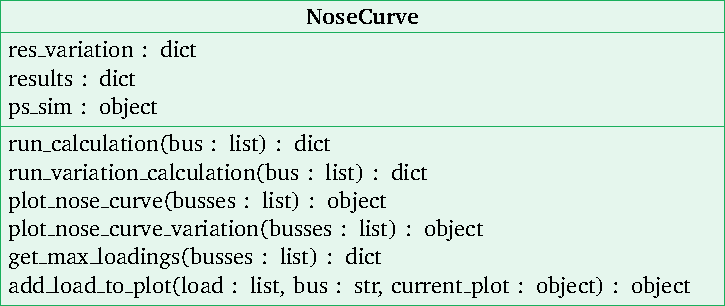
\includegraphics[width=12cm]{tikz_graphics/images/class_diagram_nosecurve_complete.pdf}
    \caption{Complete class diagram of the class Nose Curves; including all attributes and methods with data types, returns, and inputs}
    \label{fig:class-diagram-nose-curves}
\end{figure}


\subsection{Extended Class Diagram of the Class ViolationIntegral}
\subsection{Extended Class Diagram of the Class CriticalTimes}

% %%%%%%%%%%%%%%%%%%%%%%%%%%%%%%%%%%%%%%%%%%
% \section{OLTC control}


%%%%%%%%%%%%%%%%%%%%%%%%%%%%%%%%%%%%%%%%%%
%%%%%%%%%%%%%%%%%%%%%%%%%%%%%%%%%%%%%%%%%%
\chapter{Validation}
\label{app:validation}

%%%%%%%%%%%%%%%%%%%%%%%%%%%%%%%%%%%%%%%%%%
\section{Datails About Used Networks}
\label{app:networks}

\subsection{Single-Machine Infinite Bus-Bar Model}
\label{app:smib-model}

\commenting{Table with parameter details}

\subsection{SMIB Model with Additional Load}
\label{app:smib-w-load}

\commenting{Table with parameter details}


%%%%%%%%%%%%%%%%%%%%%%%%%%%%%%%%%%%%%%%%%%
\section{Additional Plots from the  Pi Model Validation}
\label{app:add-validation-plots}

\begin{figure}[H]
    \centering
    \includegraphics[width=\linewidth]{development_files/validation/data/s_n_comp_complete.pdf}
    \caption[Model results concerning the variation of the rated apparent power]{Voltage results of the $\Pi$-modeled transformer in the \acs{SMIB} model between PowerFactory and the Python framework; Variation of the rated apparent power $S_\mathrm{n}$; Left column is showing the data for the Pathon module \textit{diffpssi}, on the right the comparative tool \textit{DIgSILENT PowerFactory}}
    \label{fig:valid-s-compl}
\end{figure}

\begin{figure}[H]
    \centering
    \includegraphics[width=\linewidth]{development_files/validation/data/s_n_comp_1100mva.pdf}
    \caption{Comparison of one variation parameter between \textit{diffpssi} and \textit{DIgSILENT PowerFactory}; each plot focussing on one bus in the variation of the rated apparent power $S_\mathrm{n}$}
    \label{fig:valid-s-1100}
\end{figure}

\begin{figure}[H]
    \centering
    \includegraphics[width=\linewidth]{development_files/validation/data/theta_comp_complete.pdf}
    \caption{Comparison of the $\Pi$-modeled transformer in the \acs{SMIB} model between PowerFactory and the Python framework}
    \label{fig:valid-ratio-comp}
\end{figure}

\begin{figure}[H]
    \centering
    \includegraphics[width=\linewidth]{development_files/validation/data/theta_comp_ratio09.pdf}
    \caption{Comparison of one variation parameter between \textit{diffpssi} and \textit{DIgSILENT PowerFactory}; each plot focussing on one bus in the variation of the longitudinal transformer ratio $\vartheta$}
    \label{fig:valid-ratio-09}
\end{figure}

%%%%%%%%%%%%%%%%%%%%%%%%%%%%%%%%%%%%%%%%%%
\section{Additional Plots from the Tap Changer Control Schemes}
\label{app:add-validation-tap-changer}

\subsection{OLTC validation}

For simple load:
\begin{figure}[H]
    \centering
    \includegraphics[width=\linewidth]{development_files/validation/data/tds_oltc_simple-load.pdf}
    \caption{\acf{TDS} for standard discrete \acs{OLTC} control scheme applied to the simple load network}
    \label{fig:valid-ratio-09}
\end{figure}

For SMIB with load:
\begin{figure}[H]
    \centering
    \includegraphics[width=\linewidth]{development_files/validation/data/tds_oltc_ex-smib.pdf}
    \caption[Time Domain Result of the OLTC control scheme applied on the extended \acs{SMIB} network]{\acf{TDS} of the standard discrete \acs{OLTC} control scheme; Result of the extended or modified \acs{SMIB} model with additional load}
    \label{fig:tds-oltc-ex-smib}
\end{figure}

\begin{figure}[H]
    \centering
    \includegraphics[width=\linewidth]{development_files/validation/data/oltc_ex-smib_integrator.pdf}
    \caption{Internal signal of the standard discrete \acs{OLTC} control: The integrator signal, representing the time constant for enabling the switching operation}
    \label{fig:int-signal-oltc-ext-smib-integrator}
\end{figure}

\subsection{FSM validation}

For simple load:
\begin{figure}[H]
    \centering
    \includegraphics[width=\linewidth]{development_files/validation/data/signal_vdead_fsm_simple.pdf}
    \caption{Signal evolution for the voltage difference dependent \acs{FSM} control scheme; Plot of the deadband filtered voltage difference $v_\mathrm{dead}$ for the simple load validation case}
    \label{fig:signal-vdead-fsm-simple}
\end{figure}

For SMIB with load:

\begin{figure}[H]
    \centering
    \includegraphics[width=\linewidth]{development_files/validation/data/tds_fsm_vdiff.pdf}
    \caption[\acs{TDS} for a \acs{FSM} control scheme switching based on the voltage difference]{\acs{TDS} for a \acs{FSM} control scheme switching based on the voltage difference}
    \label{fig:tds-fsm-vdiff-ext-smib}
\end{figure}


\begin{figure}[H]
    \centering
    \includegraphics[width=\linewidth]{development_files/validation/data/tds_fsm_preferred.pdf}
    \caption[Differing \acs{TDS} for a \acs{FSM} control scheme preferring the \acs{FSM}]{Differing \acs{TDS} for a \acs{FSM} control scheme preferring the \acs{FSM}}
    \label{fig:tds-fsm-preferred}
\end{figure}

%%%%%%%%%%%%%%%%%%%%%%%%%%%%%%%%%%%%%%%%%%
%%%%%%%%%%%%%%%%%%%%%%%%%%%%%%%%%%%%%%%%%%
\chapter{Case study}